\section{Αλληλεπίδραση νέφους με Jet}
	Εφόσον έχουμε κατασκευάσει το μοντέλο ενός μοριακού νέφους μπορούμε να προχωρήσουμε στη προσομοίωση της αλληλεπίδρασης ενός πλήθους τέτοιων νεφών με έναν σχετικιστικό πίδακα υλικού (που προέρχεται από το κέντρο του γαλαξία).
	
\subsection{Ορισμός του προβλήματος}
	Όπως και προηγουμένως θα ξεκινήσουμε με ένα test problem με σχετικά μικρό αριθμό νεφών ώστε να μελετήσουμε την ευστάθεια και την αποτελεσματικότητα του κώδικα.
	
\begin{marginfigure}
	\centering
	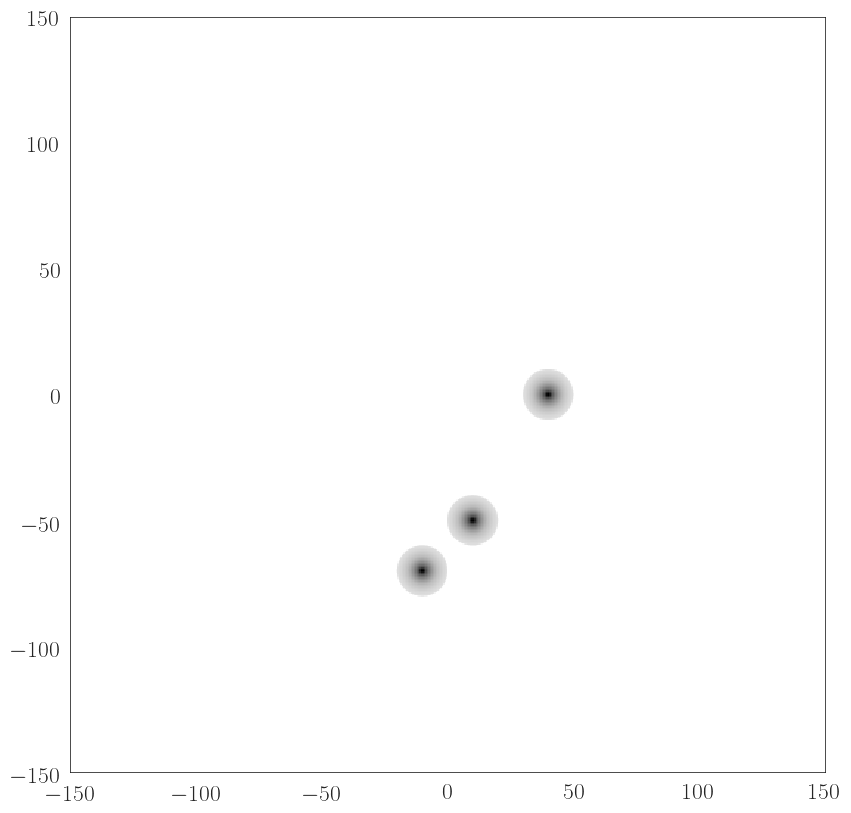
\includegraphics[width=1\linewidth]{DataImages/Jet0}
	\caption{}
	\label{fig:jet0}
\end{marginfigure}

	Έτσι ξεκινήσαμε με τη τοποθέτηση 3 μοριακών νεφών με κατανομή πυκνότητας όπως ορίστηκε στο προηγούμενο κεφάλαιο και ακτίνας \SI{10}{pc}. Τα μοριακά νέφη βρίσκονται μέσα στη μεσοαστρική ύλη με πυκνότητα \SI{1}{cm^{-3}} σε ένα τετραγωνικό χωρίο με μέγεθος \SI{300}{pc} το οποίο το χωρίζουμε σε \SI{512}{pixel}. Έτσι έχουμε μια ανάλυση των \SI{0.58}{pc}. 
	
	Για τον πίδακα χρησιμοποιούμε μια τροποποιημένη συνοριακή συνθήκη για κέντρο του κάτω σύνορο του χωρίου όπου προσδίδουμε μια σχετικιστικά ροή υλικού με πυκνότητα \SI{1e-4}{cm^{-3}} και παράγοντα lorentz $\gamma = 4$. Η διατομή της ροής είναι στα \SI{1.5}{pc}.
	
	Επειδή η χρονική κλίμακα αλληλεπίδρασης του νέφους με το πίδακα $L/c$, με $L$ τη τυπική αρχική, είναι τάξης χιλιάδων ετών δηλαδή πολύ μικρότερη από το χρόνο της βαρυτικής κατάρρευσης θεωρήσαμε τη βαρύτητα αμελητέα και έτσι επιλέξαμε να μην την ενεργοποιήσουμε.
	
	
\subsection{Σχετικιστικός Πίδακας μέσα σε Αδιατάρακτο μέσο}
	Με βάση την λύση του μονοδιάστατου προβλήματος Riemann βρίσκουμε ότι η μόνη φυσικά αποδεκτή λύση είναι αυτή που παραθέτουμε στο παρακάτω σχήμα. Από τις σχέσεις αυτές μπορούμε να υπολογίσουμε και τη θερμοκρασία για το διαταραγμένο μέσο. Έτσι βρίσκουμε για τη περιοχή μπροστά από την επιφάνεια διεπαφής  μια θερμοκρασία \SI{1e10.16}{K} και για την αντίστοιχη μετά \SI{1e13.7}{K}

\begin{marginfigure}
	\centering
	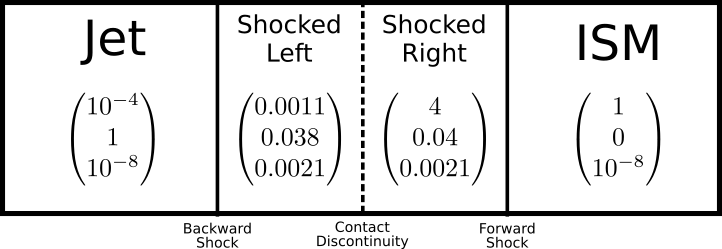
\includegraphics[width=1\linewidth]{Images/shock-shock}
	\caption{}
	\label{fig:shock-shock}
\end{marginfigure}

\begin{figure}[h]
	\centering
	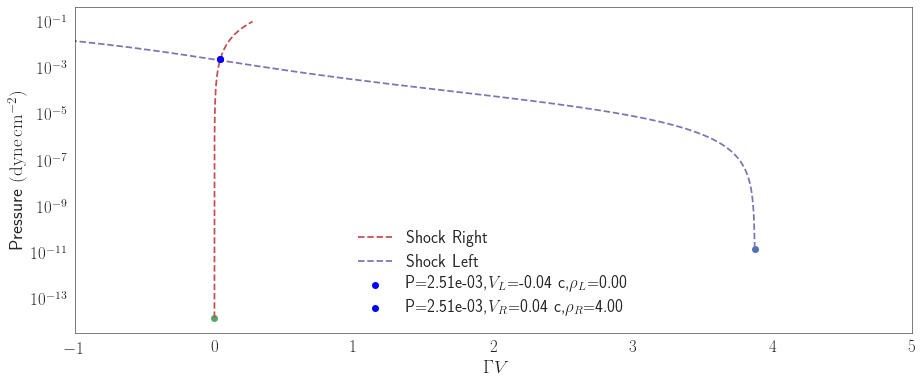
\includegraphics[width=1\linewidth]{DataImages/Shock-Shock}
	\caption{}
	\label{fig:shock-shockbl}
\end{figure}


\subsubsection{Προσομοίωση αλληλεπίδρασης με ISM}
	Στη συνέχεια παραθέτουμε τα αποτελέσματα της προσομοίωσης μας, αρχικά στο πρώτο στάδιο όπου έχουμε την αλληλεπίδραση του πίδακα με το μεσοαστρικό αέριο. Όπως φαίνεται από το σχήμα \ref{fig:rhonocool} έχουμε συμφωνία με τη προβλεπόμενη τιμή για τη πυκνότητα, το οποίο επιβεβαιώνουμε και για τις υπόλοιπες ποσότητες.
	
	
\begin{figure}[h]
	\centering
	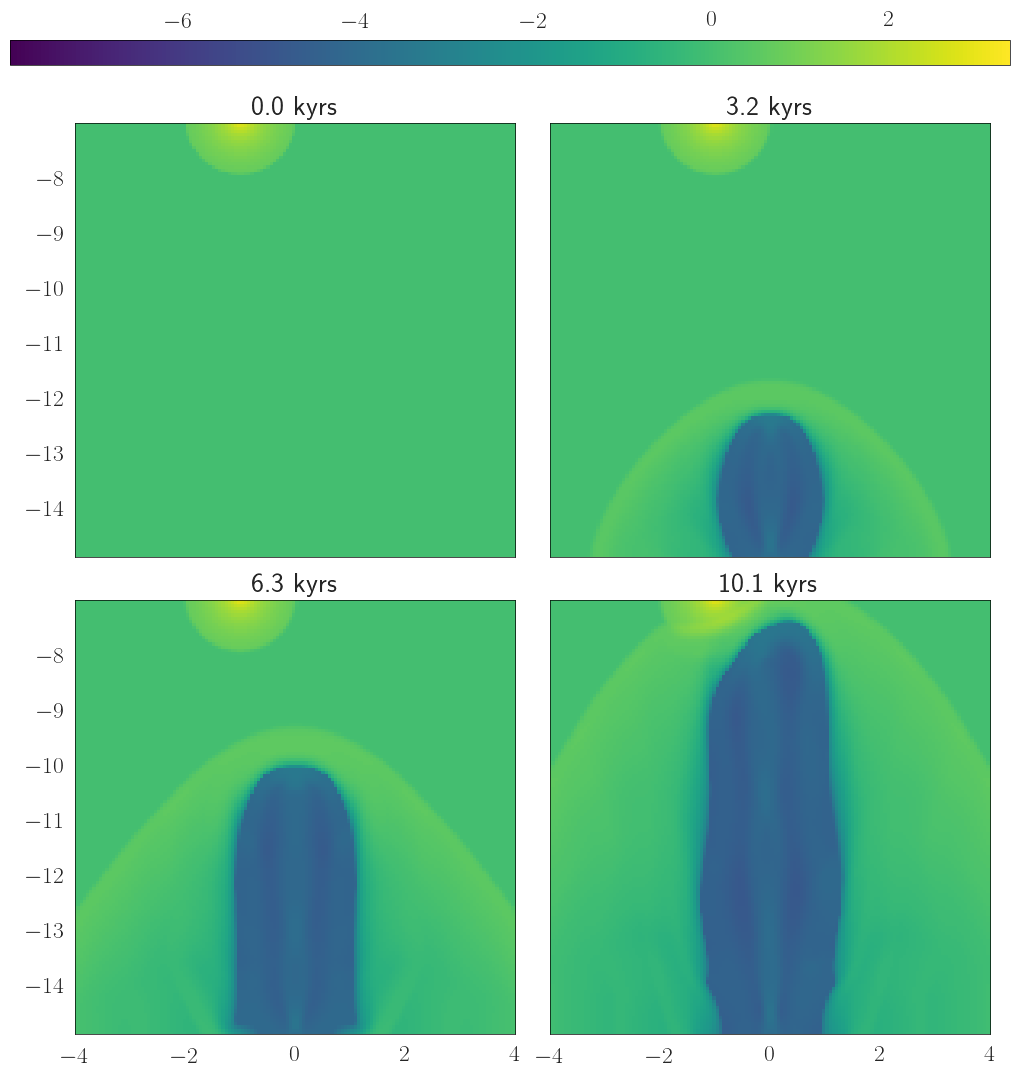
\includegraphics[width=1\linewidth]{DataImages/RHOnoCool}
	\caption{}
	\label{fig:rhonocool}
\end{figure}

\begin{figure}[h]
	\centering
	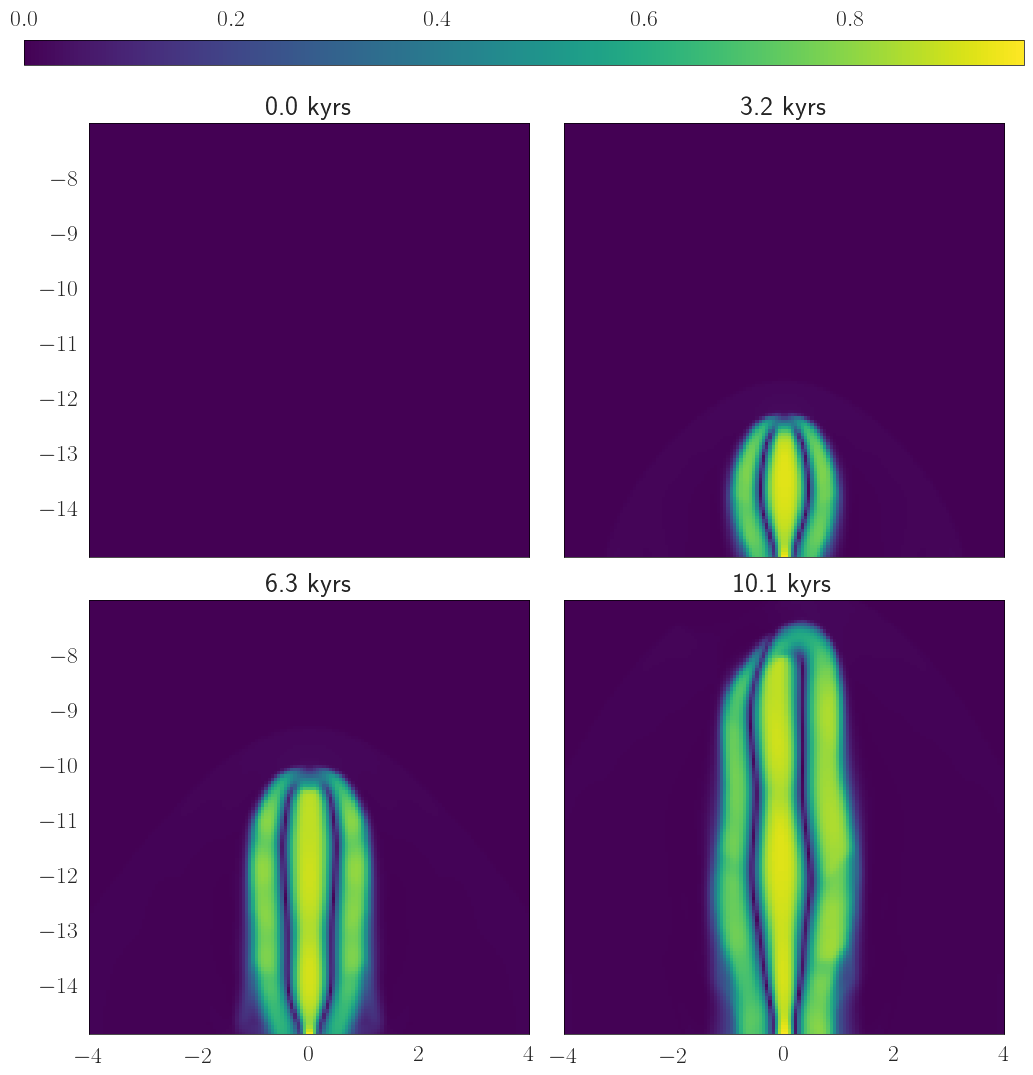
\includegraphics[width=1\linewidth]{DataImages/VnoCool}
	\caption{}
	\label{fig:vnocool}
\end{figure}



\subsubsection{Aλληλεπίδρασης με ISM και νέφος}
\begin{figure}[h]
	\centering
	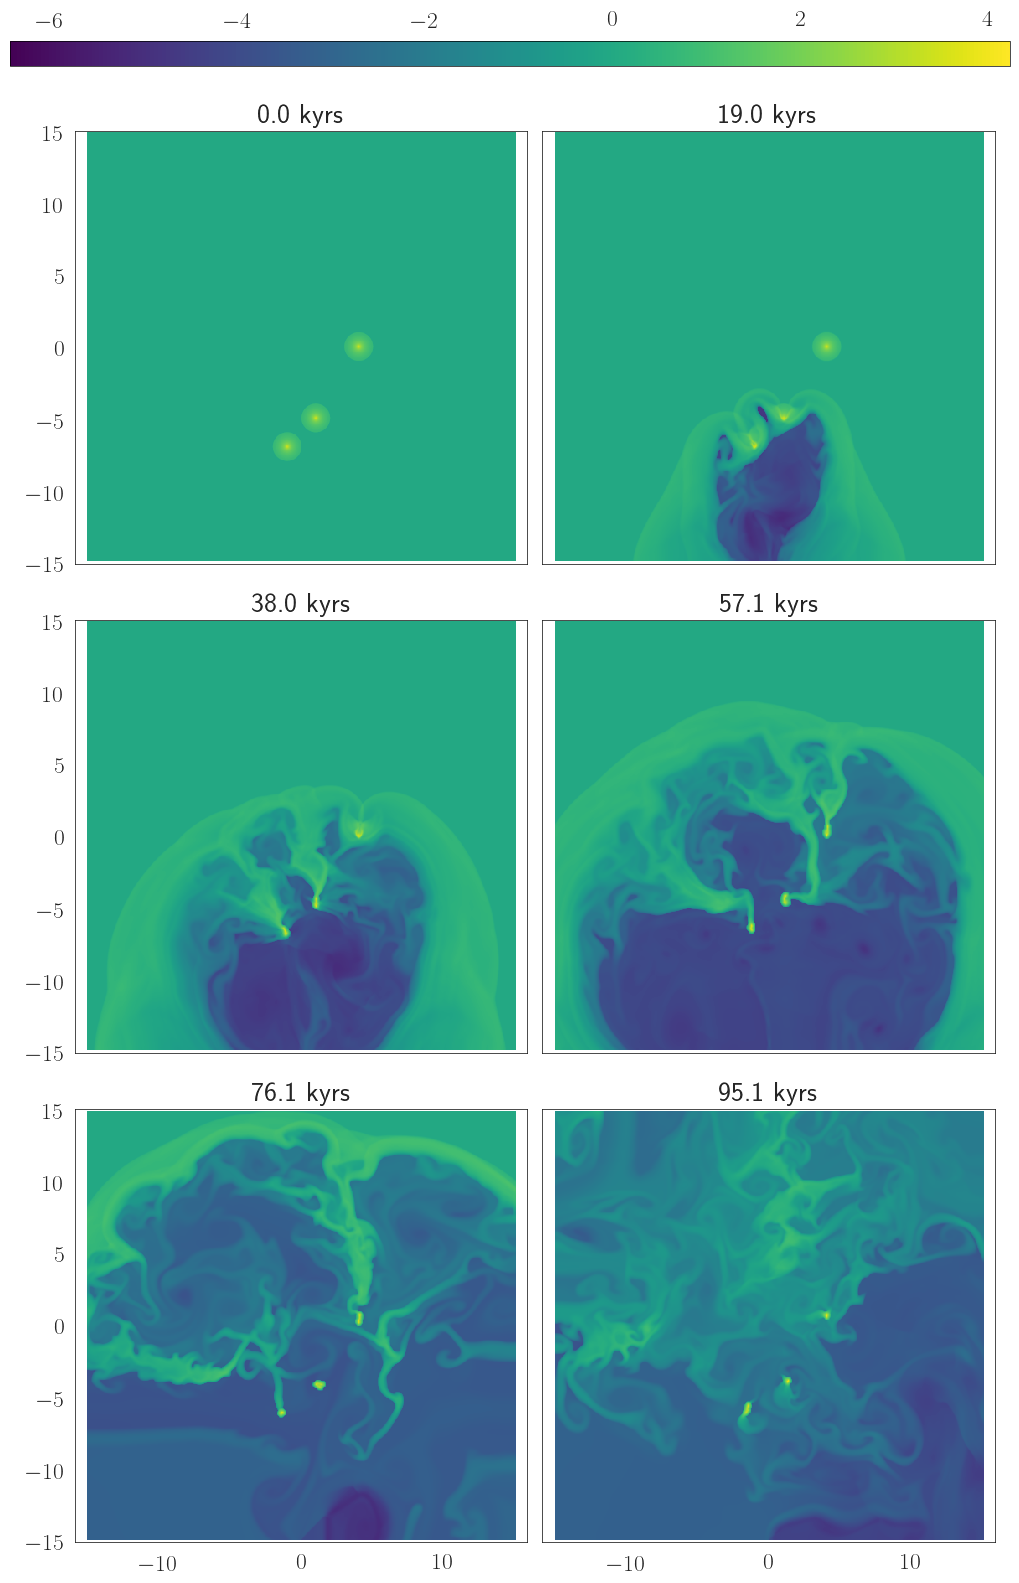
\includegraphics[width=1\linewidth]{DataImages/JetCloudRHO}
	\caption{}
	\label{fig:jetcloudrho}
\end{figure}

\begin{figure}[h]
	\centering
	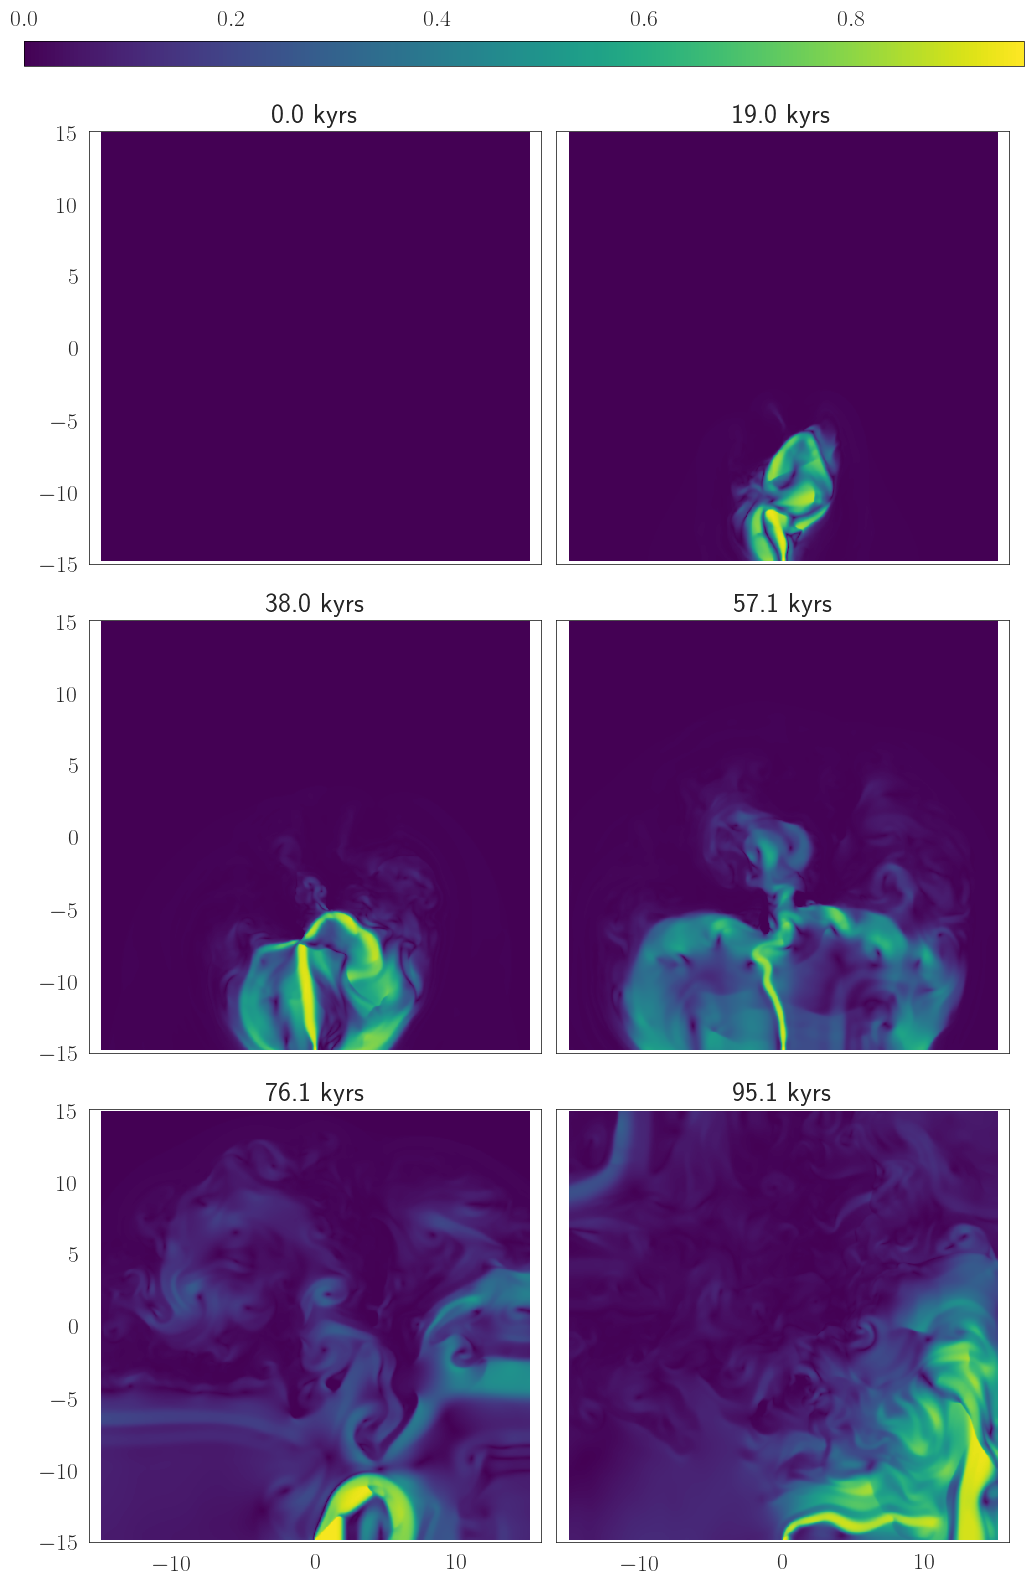
\includegraphics[width=1\linewidth]{DataImages/JetCloudV}
	\caption{}
	\label{fig:jetcloudv}
\end{figure}

Το μεγάλο ποσοστό υψηλών ταχυτήτων συμφωνεί με αντίστοιχες large-scale προσομοιώσεις (Wagner, Bicknell (2011))
\begin{itemize}
	\item{Η προσομοίωση είναι 2D}
	\item{Δεν έχουμε λάβει υπόψιν την επίδραση των μαγνητικών πεδίων}
	\item{Επίδραση από τα Boundaries}
\end{itemize}

\begin{figure}[h]
	\centering
	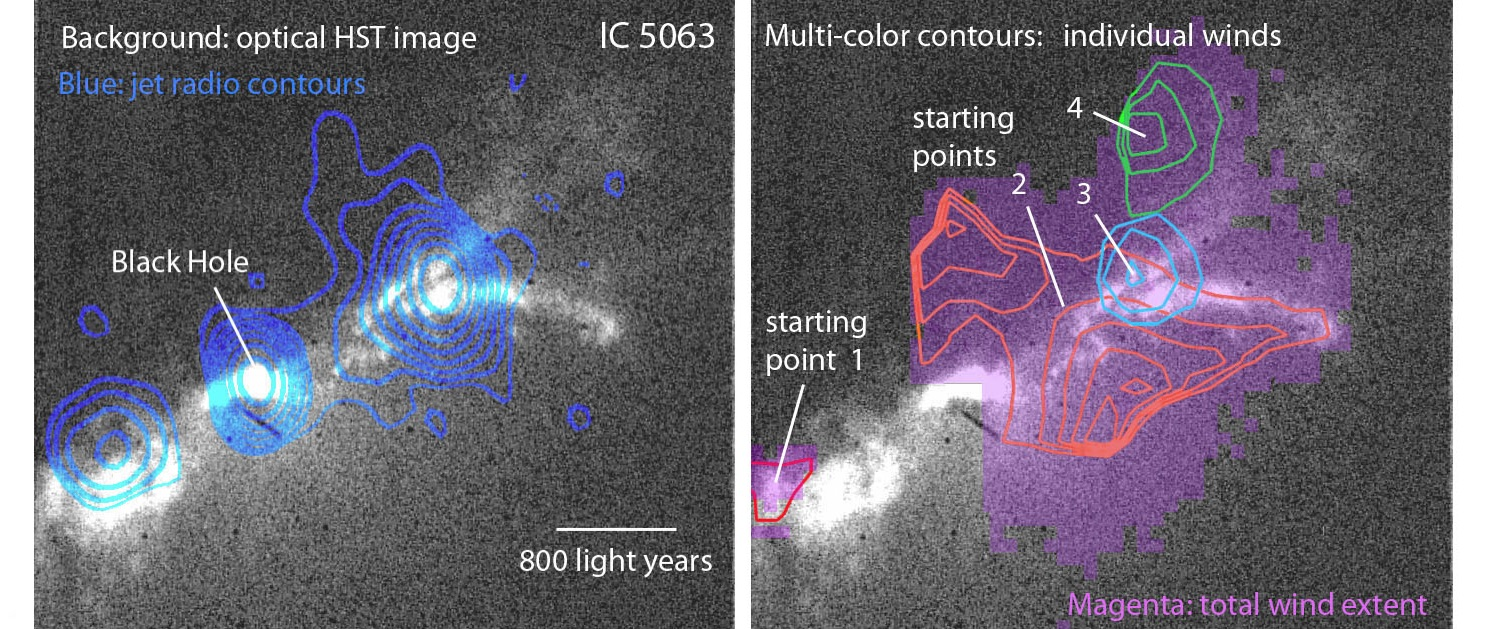
\includegraphics[width=1\linewidth]{../Presentation/Images/thejetofabla}
	\caption{}
	\label{fig:thejetofabla}
\end{figure}

